\section{Post-processing and drawing} \label{sec:ideal_exp_sno}
%------------------------------------------------------
In this section, we explain post-processing and the method of drawing the calculation result.
In the tutorial, the distributed files in \netcdf format are merged into one file
and converted into a single \netcdf file that can be read by {\grads}.
The binary form makes it easy for users to analyze the result.
Link to the post-processing tool \sno compiled in Section \ref{sec:compile_sno}:
\begin{verbatim}
  $ ln -s ../../../../../bin/sno  ./
\end{verbatim}

The method of execution of \sno is the same as that of \scalerm, i.e.,
\begin{verbatim}
 $ mpirun -n [the number of the processes] ./sno [the configuration file]
\end{verbatim}
The configuration file \verb|sample/sno_R20kmDX500m.conf| is intended for special uses of \sno.
Give this configuration file to \sno and execute it as follows:
\begin{verbatim}
  $ cp  sample/sno_R20kmDX500m.conf  ./sno_R20kmDX500m.conf
  $ mpirun  -n  2  ./sno  ./sno_R20kmDX500m.conf
\end{verbatim}
If there is no error message and the following message is displayed to the standard output,
the conversion is completed without problem:
\msgbox{
\verb|*** End   SCALE-NetCDF Operator| \\
}

The execution of \sno should be handled,
so that the number of MPI processes is identical to, or a divisor of, that used for the run of \scalerm.
The following file is generated under the same directory by this execution:
\begin{alltt}
  merged_history.pe000000.nc
\end{alltt}
The \netcdf file is the converted file obtained by merging the divided files,
and readable in \grads by ``sdfopen'' command without the ``ctl'' file.

To confirm whether the calculation is satisfactory,
draw a figure using \grads script \verb|checkfig_ideal.gs|.
Note that the grammar depends on the version of \grads.
If a warning appears, the \grads script should be rewritten appropriately:
\begin{verbatim}
  $ grads -blc checkfig_ideal.gs
\end{verbatim}
If it is successfully completed, the following files are generated:

\begin{verbatim}
   ideal_QHYD.png
   ideal_W.png
\end{verbatim}
The same figures as Fig. \ref{fig_ideal} can be found in the simulation,
and post-processing is successfully concluded.

\begin{figure}[htb]
\begin{center}
  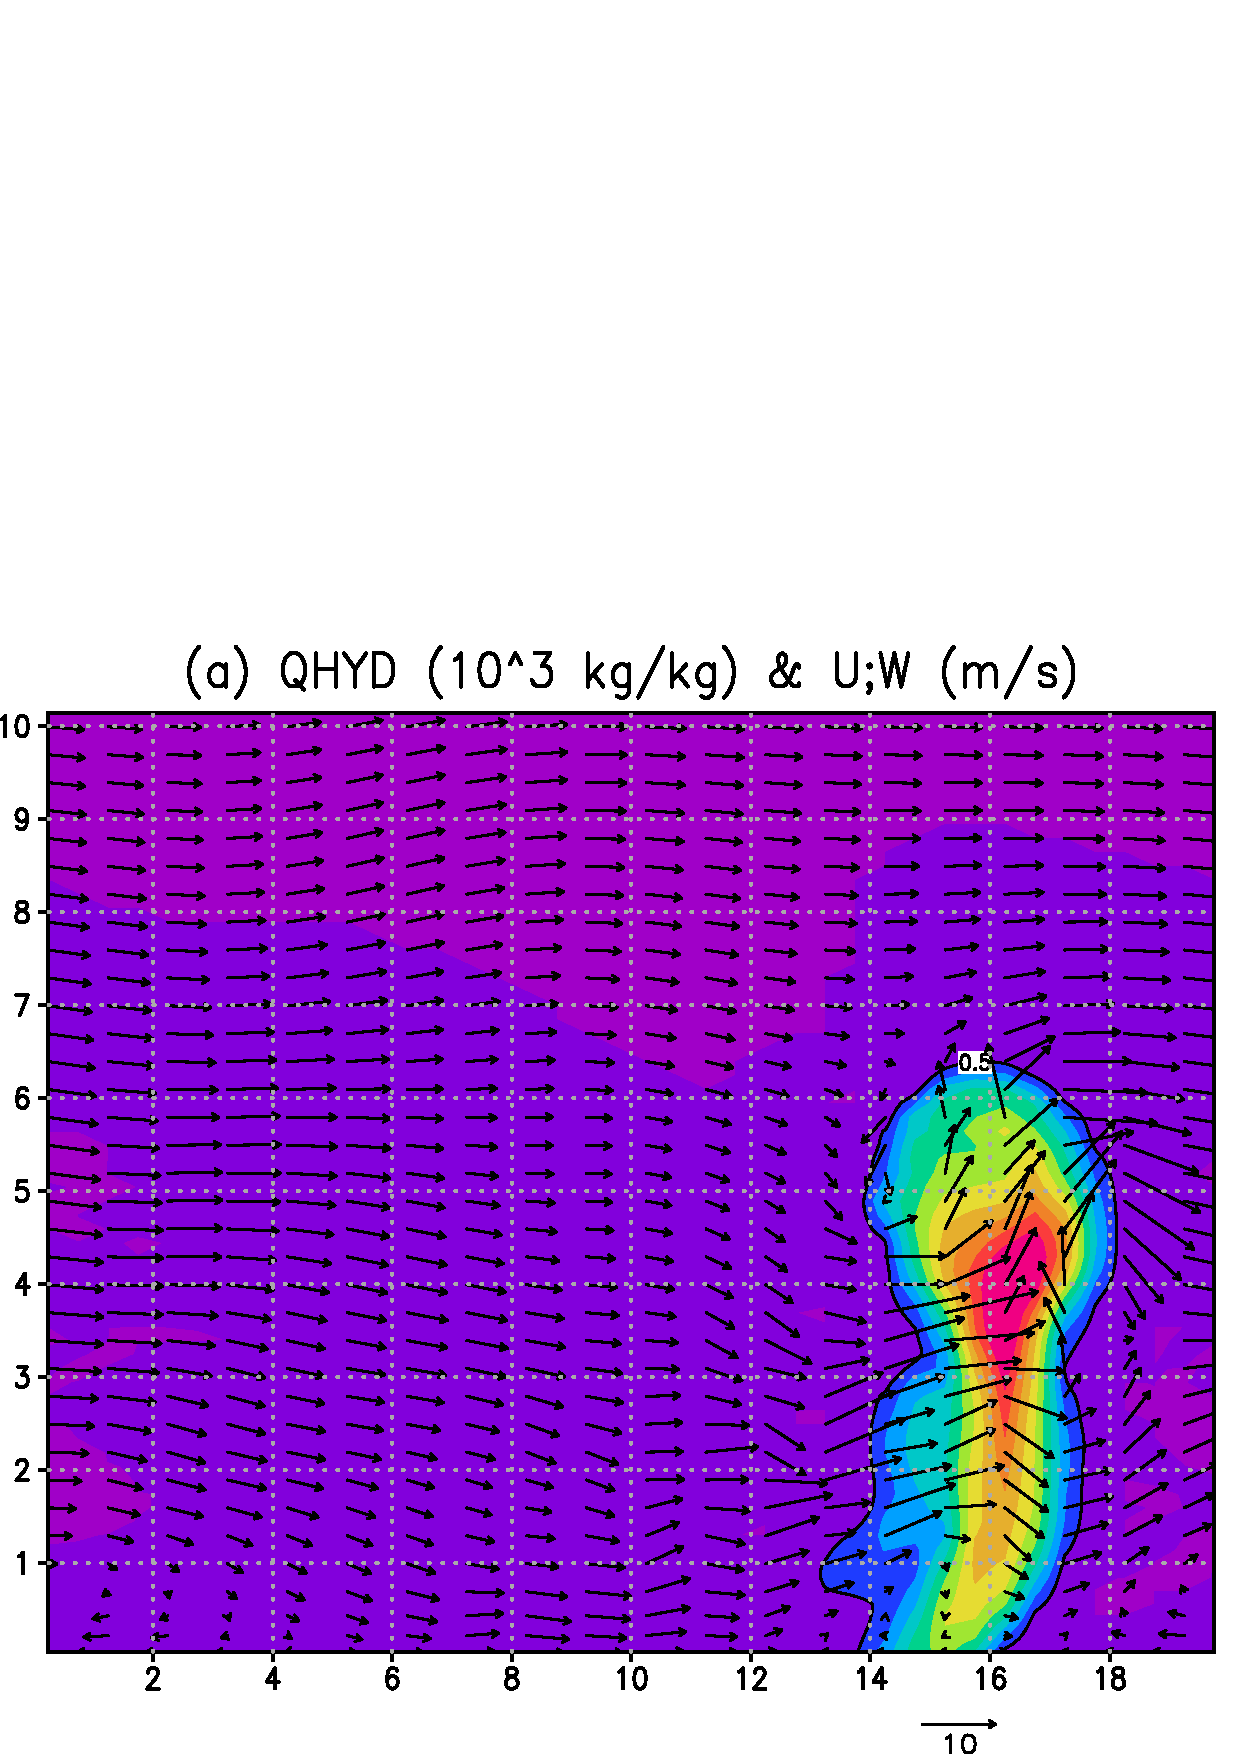
\includegraphics[width=0.65\hsize]{./../../figure/ideal_qhyd.pdf}\\
  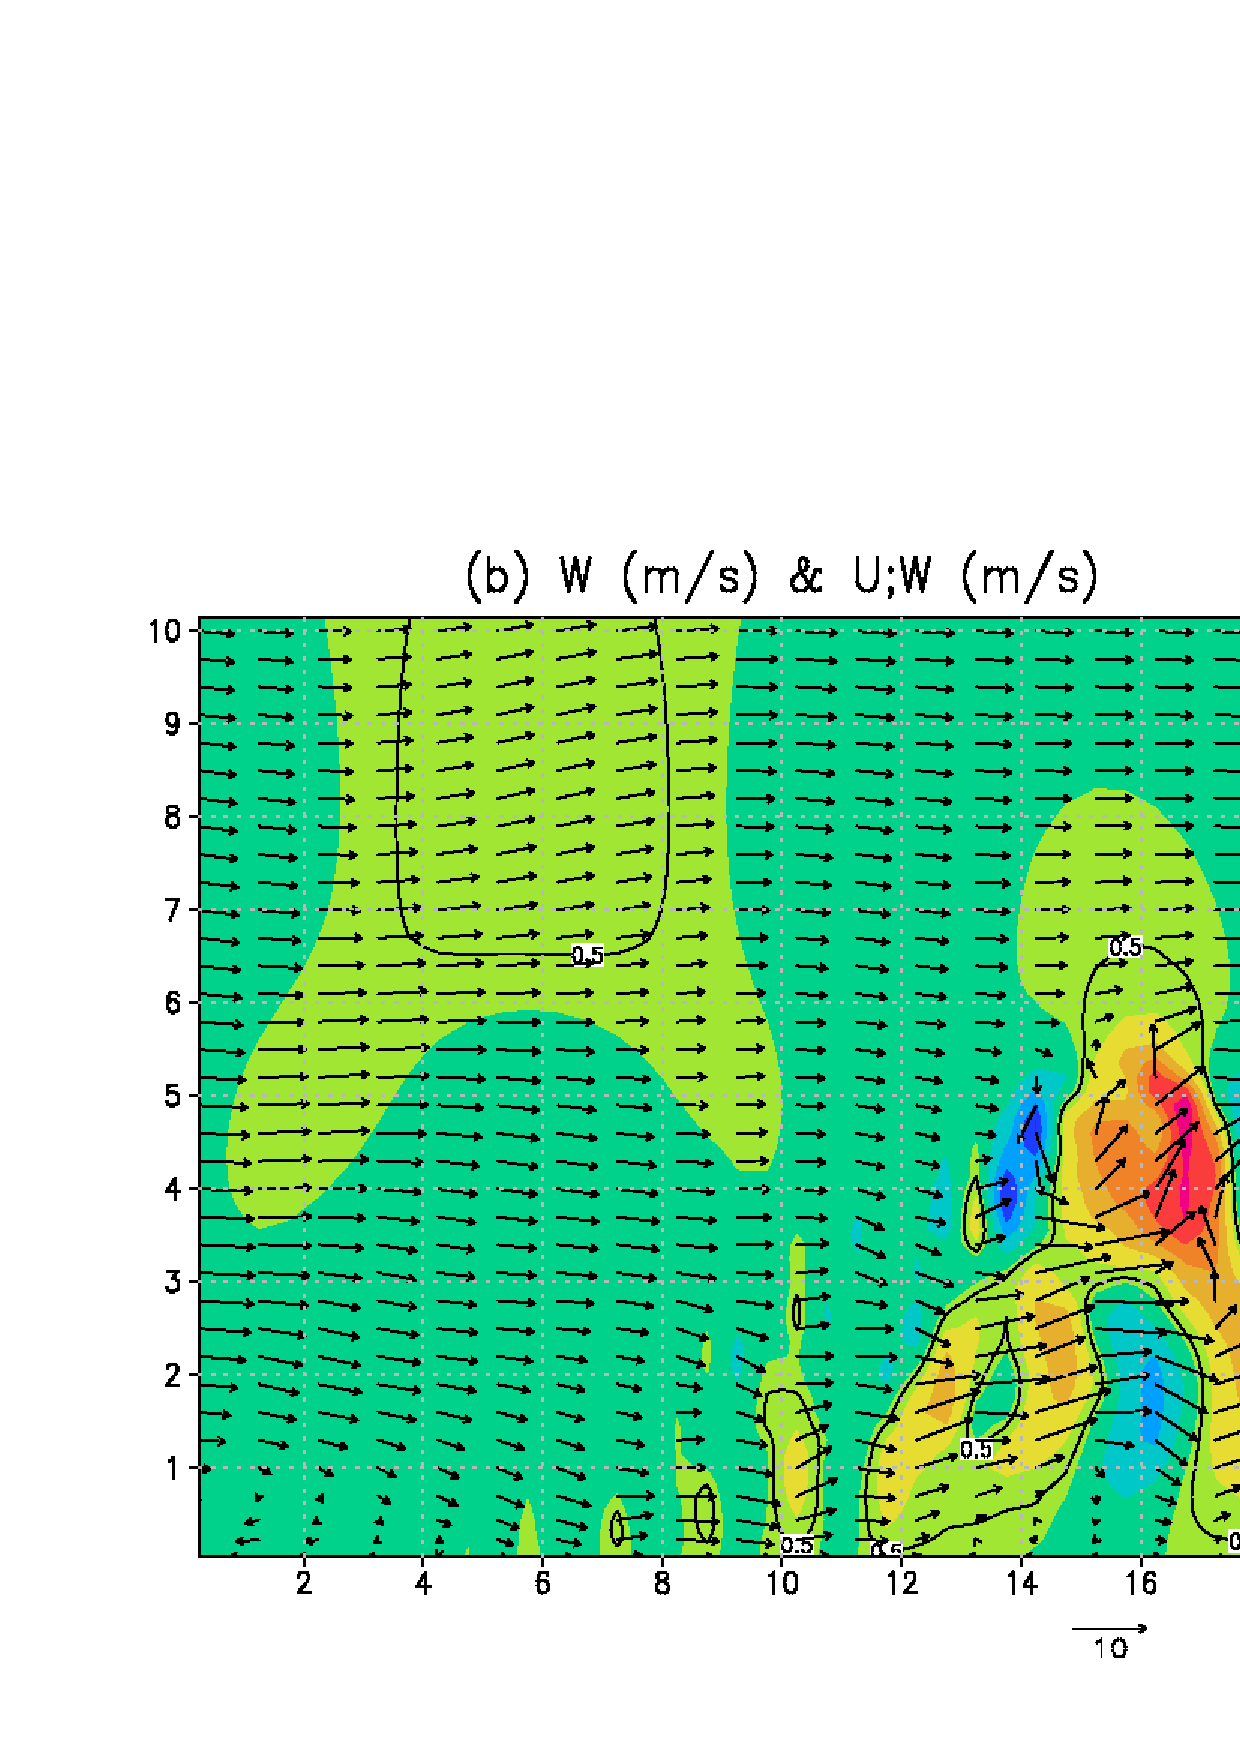
\includegraphics[width=0.65\hsize]{./../../figure/ideal_W.pdf}\\
  \caption{The horizontal-vertical cross-section after t=1200 s (20 minutes later);
            Figure (a) shows the mass concentration of the hydrometeor, and 
            Figure (b) shows the vertical velocity. 
            In both of figures, the vector indicates flow.}
  \label{fig_ideal}
\end{center}
\end{figure}

